\subsection{Fixed Positive Voltage Regulator:}

\begin{multicols}{2}
\begin{tasks}
\task {\bfseries\itshape First Circuit, IC used: 7805:}
\begin{figure}[H]
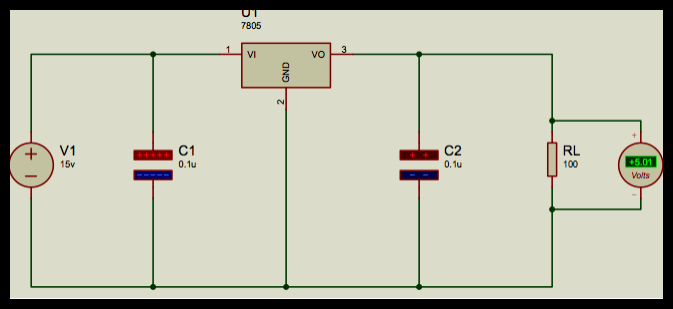
\includegraphics[scale=.36]{s4.png}
\centering \linebreak \linebreak Figure 4.2.0: LM7805 - Fixed Positive voltage regulator circuit.
\end{figure}
\begin{center}
\begin{tabular}[.5cm]{ c c }
\toprule
Source Voltage & Voltage in $R_{L}$ \\
\midrule
3.0 V & 1.72 V \\
\cmidrule{1-2}
4.0 V & 2.70 V \\
\cmidrule{1-2}
5.0 V & 3.60 V \\
\cmidrule{1-2}
6.0 V & 4.67 V \\
\cmidrule{1-2}
7.0 V & 5.0 V \\
\cmidrule{1-2}
8.0 V & 5.0 V \\
\cmidrule{1-2}
9.0 V & 5.0 V \\
\cmidrule{1-2}
10.0 V & 5.0 V \\
\cmidrule{1-2}
11.0 V & 5.0 V \\
\cmidrule{1-2}
12.0 V & 5.0 V \\
\cmidrule{1-2}
13.0 V & 5.0 V \\
\cmidrule{1-2}
14.0 V & 5.0 V \\
\cmidrule{1-2}
15.0 V & 5.0 V \\
\cmidrule{1-2}
16.0 V & 5.0 V \\
\bottomrule
\end{tabular}
\end{center} 

\task {\bfseries\itshape Second Circuit, IC used: 7812:}
\begin{figure}[H]
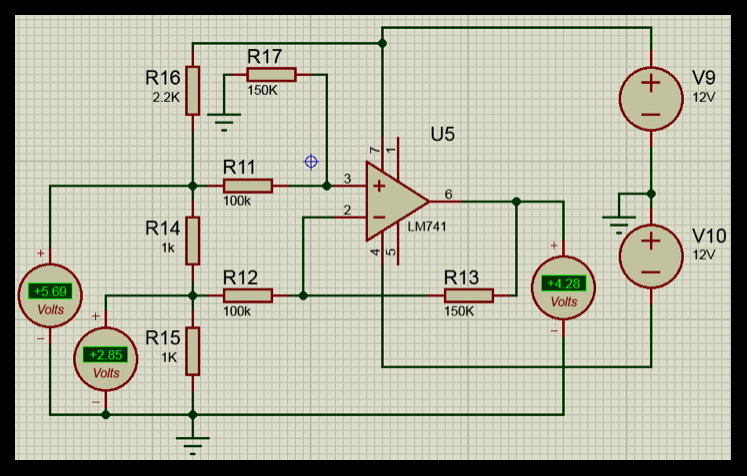
\includegraphics[scale=.355]{s5.png}
\centering \linebreak \linebreak Figure 4.2.1: LM7812 - Fixed Positive voltage regulator circuit.
\end{figure}
\begin{center}
\begin{tabular}[.5cm]{ c c }
\toprule
Source Voltage & Voltage in $R_{L}$ \\
\midrule
3.0 V & 1.72 V \\
\cmidrule{1-2}
4.0 V & 2.70 V \\
\cmidrule{1-2}
5.0 V & 3.69 V \\
\cmidrule{1-2}
6.0 V & 4.67 V \\
\cmidrule{1-2}
7.0 V & 5.66 V \\
\cmidrule{1-2}
8.0 V & 6.65 V \\
\cmidrule{1-2}
9.0 V & 7.64 V \\
\cmidrule{1-2}
10.0 V & 8.64 V \\
\cmidrule{1-2}
11.0 V & 9.63 V \\
\cmidrule{1-2}
12.0 V & 10.6 V \\
\cmidrule{1-2}
13.0 V & 11.6 V \\
\cmidrule{1-2}
14.0 V & 12.0 V \\
\cmidrule{1-2}
15.0 V & 12.0 V \\
\cmidrule{1-2}
16.0 V & 12.0 V \\
\bottomrule
\end{tabular}
\end{center} 
\end{tasks}
\end{multicols}

\pagebreak